\documentclass[notes,11pt, aspectratio=169, xcolor=table]{beamer}

\usepackage{pgfpages}
% These slides also contain speaker notes. You can print just the slides,
% just the notes, or both, depending on the setting below. Comment out the want
% you want.
\setbeameroption{hide notes} % Only slide
%\setbeameroption{show only notes} % Only notes
%\setbeameroption{show notes on second screen=right} % Both

\usepackage{helvet}
\usepackage[default]{lato}
\usepackage{array}

\newtheorem{proposition}{Proposition}
\newcommand{\blue}[1]{\textcolor{blue}{#1}}
\newcommand{\white}[1]{\textcolor{white}{#1}}

\usepackage{tikz}
\usetikzlibrary{shapes.geometric}
\usepackage{pgfplots}
\usetikzlibrary{patterns, pgfplots.fillbetween}
\usepackage{graphicx}
\usepackage{verbatim}
\setbeamertemplate{note page}{\pagecolor{yellow!5}\insertnote}
\usetikzlibrary{positioning}
\usetikzlibrary{snakes}
\usetikzlibrary{calc}
\usetikzlibrary{arrows}
\usetikzlibrary{decorations.markings}
\usetikzlibrary{shapes.misc}
\usetikzlibrary{matrix,shapes,arrows,fit,tikzmark}
\usepackage{amsmath}
\usepackage{mathpazo}
\usepackage{hyperref}
\usepackage{lipsum}
\usepackage{multimedia}
\usepackage{graphicx}
\usepackage{multirow}
\usepackage{graphicx}
\usepackage{dcolumn}
\usepackage{bbm}
\usepackage[style=authoryear,sorting=nyt,uniquename=false]{biblatex}

\addbibresource{references.bib} 

\newcolumntype{d}[0]{D{.}{.}{5}}

\def\@@mybluebox[#1][#2]#3{
    \sbox\mytempbox{#3}%
    \mytemplen\ht\mytempbox
    \advance\mytemplen #1\relax
    \ht\mytempbox\mytemplen
    \mytemplen\dp\mytempbox
    \advance\mytemplen #2\relax
    \dp\mytempbox\mytemplen
    \colorbox{myblue}{\hspace{1em}\usebox{\mytempbox}\hspace{1em}}}


\usepackage{changepage}
\usepackage{appendixnumberbeamer}
\newcommand{\beginbackup}{
   \newcounter{framenumbervorappendix}
   \setcounter{framenumbervorappendix}{\value{framenumber}}
   \setbeamertemplate{footline}
   {
     \leavevmode%
     \hline
     box{%
       \begin{beamercolorbox}[wd=\paperwidth,ht=2.25ex,dp=1ex,right]{footlinecolor}%
%         \insertframenumber  \hspace*{2ex} 
       \end{beamercolorbox}}%
     \vskip0pt%
   }
 }
\newcommand{\backupend}{
   \addtocounter{framenumbervorappendix}{-\value{framenumber}}
   \addtocounter{framenumber}{\value{framenumbervorappendix}} 
}


\usepackage{graphicx}
\usepackage[space]{grffile}
\usepackage{booktabs}

% These are my colors -- there are many like them, but these ones are mine.
\definecolor{blue}{RGB}{0,114,178}
\definecolor{red}{RGB}{213,94,0}
\definecolor{yellow}{RGB}{240,228,66}
\definecolor{green}{RGB}{0,158,115}

\hypersetup{
  colorlinks=false,
  linkbordercolor = {white},
  linkcolor = {blue}
}


%% I use a beige off white for my background
\definecolor{MyBackground}{RGB}{255,253,218}

%% Uncomment this if you want to change the background color to something else
%\setbeamercolor{background canvas}{bg=MyBackground}

%% Change the bg color to adjust your transition slide background color!
\newenvironment{transitionframe}{
  \setbeamercolor{background canvas}{bg=yellow}
  \begin{frame}}{
    \end{frame}
}

\setbeamercolor{frametitle}{fg=blue}
\setbeamercolor{title}{fg=blue}
\setbeamertemplate{footline}[frame number]
\setbeamertemplate{navigation symbols}{} 
\setbeamertemplate{itemize items}{-}
\setbeamercolor{itemize item}{fg=blue}
\setbeamercolor{itemize subitem}{fg=blue}
\setbeamercolor{enumerate item}{fg=blue}
\setbeamercolor{enumerate subitem}{fg=blue}
\setbeamercolor{button}{bg=MyBackground,fg=blue,}



% If you like road maps, rather than having clutter at the top, have a roadmap show up at the end of each section 
% (and after your introduction)
% Uncomment this is if you want the roadmap!
% \AtBeginSection[]
% {
%    \begin{frame}
%        \frametitle{Roadmap of Talk}
%        \tableofcontents[currentsection]
%    \end{frame}
% }
\setbeamercolor{section in toc}{fg=blue}
\setbeamercolor{subsection in toc}{fg=red}
\setbeamersize{text margin left=1em,text margin right=1em} 

\newenvironment{wideitemize}{\itemize\addtolength{\itemsep}{10pt}}{\enditemize}

\usepackage{environ}
\NewEnviron{videoframe}[1]{
  \begin{frame}
    \vspace{-8pt}
    \begin{columns}[onlytextwidth, T] % align columns
      \begin{column}{.58\textwidth}
        \begin{minipage}[t][\textheight][t]
          {\dimexpr\textwidth}
          \vspace{8pt}
          \hspace{4pt} {\Large \sc \textcolor{blue}{#1}}
          \vspace{8pt}
          
          \BODY
        \end{minipage}
      \end{column}%
      \hfill%
      \begin{column}{.42\textwidth}
        \colorbox{green!20}{\begin{minipage}[t][1.2\textheight][t]
            {\dimexpr\textwidth}
            Face goes here
          \end{minipage}}
      \end{column}%
    \end{columns}
  \end{frame}
}

\title[]{International Trade: Lecture 4}
\subtitle[]{Classical Ricardian Trade in General Equilibrium - Part II}
\author[Góes]
{Carlos Góes\inst{1}}
\date{Fall 2025}
\institute[GWU]{\inst{1} George Washington University }



\begin{document}

%%% TIKZ STUFF
\tikzset{   
        every picture/.style={remember picture,baseline},
        every node/.style={anchor=base,align=center,outer sep=1.5pt},
        every path/.style={thick},
        }
\newcommand\marktopleft[1]{%
    \tikz[overlay,remember picture] 
        \node (marker-#1-a) at (-.3em,.3em) {};%
}
\newcommand\markbottomright[2]{%
    \tikz[overlay,remember picture] 
        \node (marker-#1-b) at (0em,0em) {};%
}
\tikzstyle{every picture}+=[remember picture] 
\tikzstyle{mybox} =[draw=black, very thick, rectangle, inner sep=10pt, inner ysep=20pt]
\tikzstyle{fancytitle} =[draw=black,fill=red, text=white]
%%%% END TIKZ STUFF



%----------------------------------------------------------------------%
%-------------------       TITLE PAGE       ---------------------------%
%----------------------------------------------------------------------%





%----------------------------------------------------------------------%






%----------------------------------------------------------------------%
%----------------------------------------------------------------------%

%----------------------------------------------------------------------%
\frame{\titlepage}
\addtocounter{framenumber}{-1}
%----------------------------------------------------------------------%



%----------------------------------------------------------------------%
%----------------------------------------------------------------------%



\begin{frame}{Last Class: Autarky Equilibrium}
\centering
\resizebox{\textwidth}{!}{%
\begin{tabular}{lcc}
\toprule
\textbf{Variable} & \textbf{United States (US)} & \textbf{Colombia (COL)} \\
\midrule
Labor endowment $L_i$ & $300$ million & $54$ million \\
Preference parameter $\alpha_i$ & $1/2$ & $3/4$ \\
Unit labor requirement for computers $a_{i,C}$ & $3{,}000$ & $5{,}400$ \\
Unit labor requirement for roses $a_{i,R}$ & $30$ & $6$ \\
\midrule
Max computers: $L_i / a_{i,C}$ & $300\text{m}/3{,}000 = 100{,}000$ & $54\text{m}/5{,}400 = 10{,}000$ \\
Max roses: $L_i / a_{i,R}$ & $300\text{m}/30 = 10\text{m}$ & $54\text{m}/6 = 9\text{m}$ \\
\midrule
Opportunity cost $a_{i,C}/a_{i,R}$ & $3{,}000/30 = 100$ & $5{,}400/6 = 900$ \\
Demand for computers: $\alpha_i L_i / a_{i,C}$ & $0.5 \times 300\text{m}/3{,}000 = 50{,}000$ & $0.75 \times 54\text{m}/5{,}400 = 7{,}500$ \\
Demand for roses: $(1{-}\alpha_i) L_i / a_{i,R}$ & $0.5 \times 300\text{m}/30 = 5\text{m}$ & $0.25 \times 54\text{m}/6 = 2.25\text{m}$ \\
\bottomrule
\end{tabular}
}
\end{frame}

\begin{frame}{Last Class: Autarky Equilibrium}

\begin{figure}[htbp!]

% California
\begin{subfigure}{}
\resizebox{0.48\textwidth}{!}{%
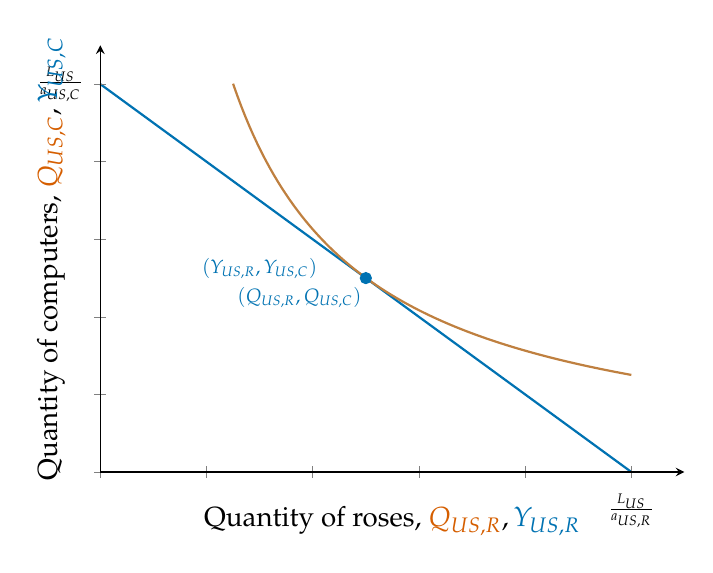
\begin{tikzpicture}
\pgfmathsetmacro{\aC}{100}       % unit labor requirement for computers
\pgfmathsetmacro{\aR}{1}         % unit labor requirement for roses
\pgfmathsetmacro{\alpha}{0.5}    % preference for computers
\pgfmathsetmacro{\Lendow}{10}    % labor endowment

% Compute equilibrium quantities
\pgfmathsetmacro{\Qc}{(\alpha*\Lendow)/\aC}
\pgfmathsetmacro{\Qr}{((1 - \alpha)*\Lendow)/\aR}

% Compute utility level
\pgfmathsetmacro{\U}{(\Qc^(\alpha))*(\Qr^(1 - \alpha))}

% Compute prefactor for indifference curve: Qc = A * Qr^(- (1 - alpha)/alpha)
\pgfmathsetmacro{\expo}{(1 - \alpha)/\alpha}
\pgfmathsetmacro{\A}{\U^(1/\alpha)}

\centering
\begin{axis}[
    ylabel={Quantity of computers, $\textcolor{red}{Q_{US,C}}, \textcolor{blue}{Y_{US,C}}$},
    xlabel={Quantity of roses, $\textcolor{red}{Q_{US,R}}, \textcolor{blue}{Y_{US,R}}$},
    ymin=0, ymax=0.11,
    xmin=0, xmax=11,
    yticklabel=\empty,
    xticklabel=\empty,
    axis lines=left,
    enlargelimits=false,
    clip=false,
    axis on top,
    scaled x ticks=false,
    width=9cm, height=7cm,
    title style={font=\bfseries}
]

% PPF: Q_C = (L/a_C) - (a_R/a_C) * Q_R
\addplot[thick, blue, domain=0:10] {\Lendow/\aC - (\aR/\aC)*x};

% Indifference curve through optimal bundle
\addplot[thick, brown, domain=2.5:10, samples=100] {\A * x^(-\expo)};

% Labels
%\node at (axis cs:3.5,0.03) {\Large $\mathcal{Y}_{US}$};
\node at (axis cs:\Lendow/\aR,-.01) {\scriptsize $\frac{L_{US}}{a_{US,R}}$};
\node at (axis cs:-.75,\Lendow/\aC) {\scriptsize $\frac{L_{US}}{a_{US,C}}$};


% Equilibrium point
\addplot[only marks, mark=*, color=blue, mark size=2pt] coordinates {(\Qr, \Qc)};
\node at (axis cs:\Qr - 1.25,\Qc - 0.005) {\scriptsize $\textcolor{blue}{(Q_{US,R},Q_{US,C})}$};
\node at (axis cs:\Qr - 2,\Qc + 0.0025) {\scriptsize $\textcolor{blue}{(Y_{US,R},Y_{US,C})}$};



\end{axis}

\end{tikzpicture}
}
\end{subfigure}
%
% Colombia
\begin{subfigure}{}
\resizebox{0.48\textwidth}{!}{%

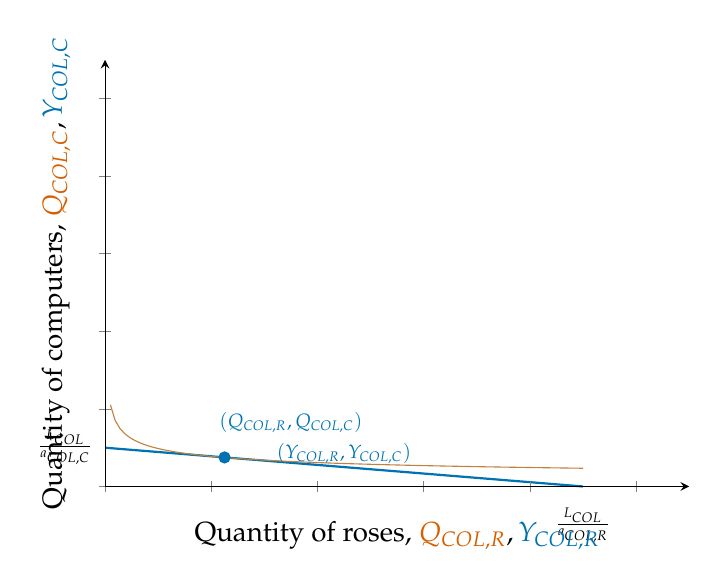
\begin{tikzpicture}
\pgfmathsetmacro{\aC}{900}       % unit labor requirement for computers
\pgfmathsetmacro{\aR}{1}         % unit labor requirement for roses
\pgfmathsetmacro{\alpha}{0.75}    % preference for computers
\pgfmathsetmacro{\Lendow}{9}    % labor endowment

% Compute equilibrium quantities
\pgfmathsetmacro{\Qc}{(\alpha*\Lendow)/\aC}
\pgfmathsetmacro{\Qr}{((1 - \alpha)*\Lendow)/\aR}

% Compute utility level
\pgfmathsetmacro{\U}{(\Qc^(\alpha))*(\Qr^(1 - \alpha))}

% Compute prefactor for indifference curve: Qc = A * Qr^(- (1 - alpha)/alpha)
\pgfmathsetmacro{\expo}{(1 - \alpha)/\alpha}
\pgfmathsetmacro{\A}{\U^(1/\alpha)}

\centering
\begin{axis}[
    ylabel={Quantity of computers, $\textcolor{red}{Q_{COL,C}}, \textcolor{blue}{Y_{COL,C}}$},
    xlabel={Quantity of roses, $\textcolor{red}{Q_{COL,R}}, \textcolor{blue}{Y_{COL,R}}$},
    ymin=0, ymax=0.11,
    xmin=0, xmax=11,
    yticklabel=\empty,
    xticklabel=\empty,
    axis lines=left,
    enlargelimits=false,
    clip=false,
    axis on top,
    scaled x ticks=false,
    width=9cm, height=7cm,
    title style={font=\bfseries}
]

% PPF: Q_C = (L/a_C) - (a_R/a_C) * Q_R
\addplot[thick, blue, domain=0:9] {\Lendow/\aC - (\aR/\aC)*x};

% Indifference curve through optimal bundle
\addplot[brown, domain=0.1:9, samples=100] {\A * x^(-\expo)};

% Labels

%\node at (axis cs:3.5,0.03) {\Large $\mathcal{Y}_{US}$};
\node at (axis cs:\Lendow/\aR,-.01) {\scriptsize $\frac{L_{COL}}{a_{COL,R}}$};
\node at (axis cs:-.75,\Lendow/\aC) {\scriptsize $\frac{L_{COL}}{a_{COL,C}}$};


% Equilibrium point
\addplot[only marks, mark=*, color=blue, mark size=2pt] coordinates {(\Qr, \Qc)};
\node at (axis cs:\Qr + 1.25,\Qc + 0.009) {\scriptsize $\textcolor{blue}{(Q_{COL,R},Q_{COL,C})}$};
\node at (axis cs:\Qr + 2.25,\Qc + 0.001) {\scriptsize $\textcolor{blue}{(Y_{COL,R},Y_{COL,C})}$};


\end{axis}

\end{tikzpicture}
}

\end{subfigure}

\caption{Autarky equilibrium}\label{fig: autarky-num}

\end{figure}
\end{frame}

\section{Trade Definitions}

\begin{frame}{Absolute and Comparative Advantage}

\begin{wideitemize}
    \item We say Colombia has an \textcolor{blue}{absolute advantage} in the production of good $p$ if $a_{COL,p} < a_{US,p}$

    \item English: absolute advantage in production = uses less labor to produce one unit \\
    \qquad \textcolor{gray}{(i.e., it is more productive)}

    \item \textcolor{blue}{Opportunity cost}: cost of producing a good, measured in foregone output of all others.

    \item \blue{Comparative advantage}: An economy has a comparative advantage in producing a good if its opportunity cost of the good is lower than in the rest of the world.

\end{wideitemize}

\end{frame}


\begin{frame}{Absolute and Comparative Advantage}

\begin{wideitemize}

    \item We say Colombia has an \textcolor{blue}{comparative advantage} in the production of roses, since:
    
    \begin{equation*}
        1/900 = a_{COL,R}/a_{COL,C} < a_{US,R}/a_{US,C} = 1/100
    \end{equation*}

    \item We say the US has an \textcolor{blue}{comparative advantage} in the production of computers, since:
    
    \begin{equation*}
        900 = a_{COL,C}/a_{COL,R
        } > a_{US,C}/a_{US,R} = 100
    \end{equation*}

\end{wideitemize}

\end{frame}

\section{Supply}

\begin{frame}{Prices under Autarky}

\begin{wideitemize}

    \item Without trade, prices reflect opportunity cost:
    \begin{itemize}
        \item In the US: $a_{US,R}/a_{US,C} = P_{US,R}/P_{US,C}$
        \item In Colombia: $a_{COL,R}/a_{COL,C} = P_{COL,R}/P_{COL,C}$
    \end{itemize}

    \item<2-> Under free trade, there are world prices, i.e. $P_R,P_C$ that hold both in countries. 

    \item<3-> If $P_R/P_C = a_{COL,R}/a_{COL,C}$, Colombian producers indifferent
    \begin{itemize}
        \item Production of computers $Y_{COL,C}$ can range from 0 to 10,000 
        \item Production of roses $Y_{COL,R}$ can range from 0 to 9mi 
    \end{itemize}

    \item<4-> If $P_R/P_C = a_{US,R}/a_{US,C}$, US producers indifferent
    \begin{itemize}
        \item Production of computers $Y_{US,C}$ can range from 0 to 100,000 
        \item Production of roses $Y_{US,R}$ can range from 0 to 10mi 
    \end{itemize}

\end{wideitemize}

\end{frame}


\begin{frame}{Prices consistent with trade}

\begin{wideitemize}

    \item In this model, \blue{countries specialize in goods in which they have a comparative advantage}:
    
    \begin{itemize}
        \item \blue{Colombia} specializes in \blue{roses} if $a_{COL,R}/a_{COL,C} < P_R/P_C$
        \item The \blue{US} specializes in \blue{computers} if $a_{US,R}/a_{US,C} > P_R/P_C$
    \end{itemize}

    \item<2-> Why? \\
        \qquad \textcolor{gray}{(relative marginal revenue is greater than its relative marginal cost)}

    \item<3-> Each country specializes in the good in which they have a comparative advantage in if:

    \begin{equation*}\label{eq: price-trade}
        \frac{a_{US,C}}{a_{US,R}} < \frac{P_C}{P_R} < \frac{a_{COL,C}}{a_{COL,R}}
    \end{equation*}
    

\end{wideitemize}

\end{frame}

\begin{frame}{Global Supply Curve}
    \begin{figure}[htpd!]
\centering
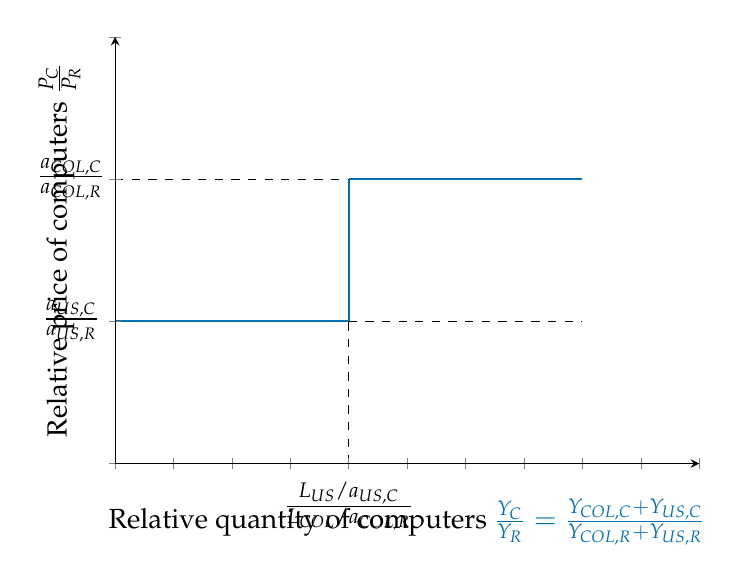
\begin{tikzpicture}
\begin{axis}[
    ylabel={Relative price of computers $\frac{P_C}{P_R}$},
    xlabel={Relative quantity of computers $\textcolor{blue}{\frac{Y_{C}}{Y_{R}} = \frac{Y_{COL,C}+Y_{US,C}}{Y_{COL,R}+Y_{US,R}} }$},
    ymin=0, ymax=3,
    xmin=0, xmax=2,
    yticklabel=\empty,
    xticklabel=\empty,
    axis lines=left,
    enlargelimits=false,
    clip=false,
    axis on top,
    scaled x ticks=false,
    width=9cm, height=7cm,
    title style={font=\bfseries}]

% Relative Supply RS
\addplot[thick, blue] coordinates {(0,1) (0.8,1.0)};
\addplot[thick, blue] coordinates {(0.8,1.0) (0.8,2.0)};
\addplot[thick, blue] coordinates {(0.8,2.0) (1.6,2.0)};
%\node at (axis cs:1.65,2.7) {\small $RS$};

% Dashed lines for autarky prices
\addplot[dashed] coordinates {(0,2.0) (0.8,2.0)};
\node at (axis cs:-0.15,2) {$\frac{a_{COL,C}}{a_{COL,R}}$};

\addplot[dashed] coordinates {(0.8,1.0) (1.6,1.0)};
\node at (axis cs:-0.15,1) {$\frac{a_{US,C}}{a_{US,R}}$};


% Vertical dashed lines for quantities
\addplot[dashed] coordinates {(0.8,0) (0.8,1.0)};
\node at (axis cs:0.8,-0.3) {$\frac{L_{US}/a_{US,C}}{L_{COL}/a_{COL,R}}$};

\end{axis}
\end{tikzpicture}
\caption{Relative Supply of Computers as a function of Relative Prices}\label{fig: relative-supply}
\end{figure}

\end{frame}

\section{Price determination}

\begin{frame}{Price Determination (i)}
\begin{wideitemize}
   

\item How are prices determined in a free trade equilibrium? \\
\qquad \textcolor{gray}{(relative prices will adjust to make sure that the global supply = global demand)}

\item<2-> \blue{Global supply}:

\begin{itemize}
    \item US fully specializes in computers: $Y^T_{C} = L_{US}/a_{US,C} = 100{,}000$
    \item Colombia fully specializes in roses? $Y^T_R = L_{COL}/a_{COL,R} = 9{,}000{,}000$. 
\end{itemize}
    
\item<3-> \blue{Global demand}:
\begin{eqnarray*}
    Q_{C} &\equiv& Q^T_{US,C} +  Q^T_{COL,C} = \alpha_{US} \frac{w_{US} L_{US} }{P_C} + \alpha_{COL} \frac{w_{COL} L_{COL} }{P_C}  \\
    Q_{R} &\equiv& Q^T_{US,R} +  Q^T_{COL,R}  = (1-\alpha_{US}) \frac{w_{US} L_{US} }{P_R} + (1-\alpha_{COL}) \frac{w_{COL} L_{COL} }{P_R}    
\end{eqnarray*}

\item<3-> Note that global demand \textcolor{red}{$Q_C/Q_R$} is decreasing in relative prices $P_C / P_R$ 
\end{wideitemize}
    
\end{frame}


\begin{frame}{Global Supply and Demand}

\begin{figure}[htpd!]
\centering
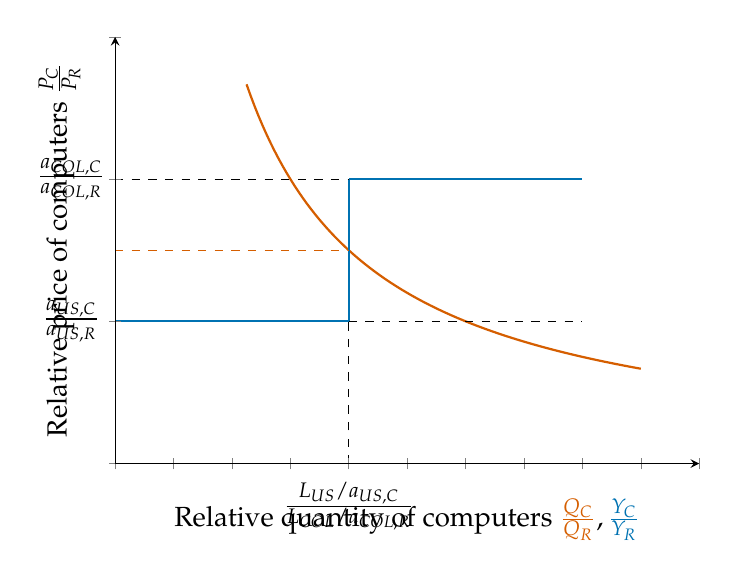
\begin{tikzpicture}
\begin{axis}[
    ylabel={Relative price of computers $\frac{P_C}{P_R}$},
    xlabel={Relative quantity of computers $\textcolor{red}{\frac{Q_{C}}{Q_{R}} } , \textcolor{blue}{\frac{Y_{C}}{Y_{R}} }$},
    ymin=0, ymax=3,
    xmin=0, xmax=2,
    yticklabel=\empty,
    xticklabel=\empty,
    axis lines=left,
    enlargelimits=false,
    clip=false,
    axis on top,
    scaled x ticks=false,
    width=9cm, height=7cm,
    title style={font=\bfseries}]

% Relative Demand RD
\addplot[
    red, thick,
    domain=0.45:1.8,
    samples=100
] {1.2/(x)};
%\node[red] at (axis cs:1.4,1.25) {\small $RD$};

% Relative Supply RS
\addplot[thick, blue] coordinates {(0,1) (0.8,1.0)};
\addplot[thick, blue] coordinates {(0.8,1.0) (0.8,2.0)};
\addplot[thick, blue] coordinates {(0.8,2.0) (1.6,2.0)};
%\node at (axis cs:1.65,2.7) {\small $RS$};

% Dashed lines for autarky prices
\addplot[dashed] coordinates {(0,2.0) (0.8,2.0)};
\node at (axis cs:-0.15,2) {$\frac{a_{COL,C}}{a_{COL,R}}$};

\addplot[dashed] coordinates {(0.8,1.0) (1.6,1.0)};
\node at (axis cs:-0.15,1) {$\frac{a_{US,C}}{a_{US,R}}$};

\addplot[dashed, red] coordinates {(0,1.5) (0.8,1.5)};

% Vertical dashed lines for quantities
\addplot[dashed] coordinates {(0.8,0) (0.8,1.0)};
\node at (axis cs:0.8,-0.3) {$\frac{L_{US}/a_{US,C}}{L_{COL}/a_{COL,R}}$};

\end{axis}
\end{tikzpicture}
\caption{Relative Supply and Demand of Computers as a Function of Relative Prices}
\end{figure}

\end{frame}


\begin{frame}{Price determination (ii)}
    \begin{wideitemize}
    \item What is $w_{US}$, $w_{COL}$?
    
    \item Countries fully specialize: only one sector operating in each country
    
    \item Wages = marginal product of each worker in the sector they are working

    \begin{equation*}
        w_{US} = P_{C} / a_{US,C}, \qquad w_{COL} = P_{R} / a_{COL,R}
    \end{equation*}
    
    \end{wideitemize}
\end{frame}

\begin{frame}{Price determination (iii)}
    \begin{wideitemize}
    \item How to get $P_C/P_R$? Trade balances, so value of exports = value of imports:
    {\scriptsize
    \begin{equation*}
        P_C ( Y_{US,C} - Q^T_{US,C}) = P_R (Y_{COL,R} - Q^T_{COL,R})
    \end{equation*}
    }
    \onslide<2->{
    {\scriptsize
    \begin{equation*}
    P_C \left( \frac{L_{US}}{a_{US,C}} - \alpha_{US} \frac{w_{US} L_{US}}{P_C} \right) = P_R \left( \frac{L_{COL}}{a_{COL,R}} - (1-\alpha_{COL}) \frac{w_{COL} L_{COL}}{P_R} \right)
    \end{equation*}
    }
    \onslide<3->{
    {\scriptsize
    \begin{equation*}    
        P_C \left( \frac{L_{US}}{a_{US,C}} - \alpha_{US} \frac{L_{US}}{a_{US,C}} \right) = P_R \left( \frac{L_{COL}}{a_{COL,R}} - (1-\alpha_{COL}) \frac{L_{COL}}{a_{COL,R}} \right)
    \end{equation*}
    }
    }
    }
    \normalsize
    \item<4-> Solving for $P_C/P_R$:
    \begin{center}
        \boxed{
        \frac{P_C}{P_R} = \frac{\alpha_{COL}}{1-\alpha_{US}} \times \frac{L_{COL}/a_{COL,R}}{L_{US}/a_{US,C}} = \frac{3/4}{1/2} \times \frac{54m / 6}{300m / 3{,}000} = 135 
        }    
    \end{center}
        
    \end{wideitemize}
\end{frame}

\begin{frame}{Production Possibilities Frontier + Trade Prices}
\begin{center}

\begin{figure}[htbp]

% California
\begin{subfigure}{}
\resizebox{0.48\linewidth}{!}{%
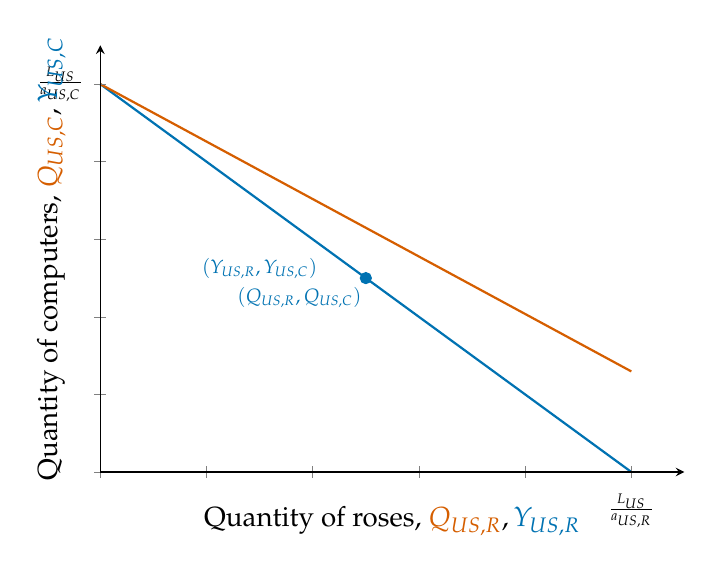
\begin{tikzpicture}
\pgfmathsetmacro{\aC}{100}       % unit labor requirement for computers
\pgfmathsetmacro{\aR}{1}         % unit labor requirement for roses
\pgfmathsetmacro{\alpha}{0.5}    % preference for computers
\pgfmathsetmacro{\Lendow}{10}    % labor endowment

% Compute equilibrium quantities
\pgfmathsetmacro{\Qc}{(\alpha*\Lendow)/\aC}
\pgfmathsetmacro{\Qr}{((1 - \alpha)*\Lendow)/\aR}

% Compute utility level
\pgfmathsetmacro{\U}{(\Qc^(\alpha))*(\Qr^(1 - \alpha))}

% Compute prefactor for indifference curve: Qc = A * Qr^(- (1 - alpha)/alpha)
\pgfmathsetmacro{\expo}{(1 - \alpha)/\alpha}
\pgfmathsetmacro{\A}{\U^(1/\alpha)}

\centering
\begin{axis}[
    ylabel={Quantity of computers, $\textcolor{red}{Q_{US,C}}, \textcolor{blue}{Y_{US,C}}$},
    xlabel={Quantity of roses, $\textcolor{red}{Q_{US,R}}, \textcolor{blue}{Y_{US,R}}$},
    ymin=0, ymax=0.11,
    xmin=0, xmax=11,
    yticklabel=\empty,
    xticklabel=\empty,
    axis lines=left,
    enlargelimits=false,
    clip=false,
    axis on top,
    scaled x ticks=false,
    width=9cm, height=7cm,
    title style={font=\bfseries}
]

% PPF: Q_C = (L/a_C) - (a_R/a_C) * Q_R
\addplot[thick, blue, domain=0:10] {\Lendow/\aC - (\aR/\aC)*x};

\addplot[thick, red, domain=0:10] {\Lendow/\aC - (1/135)*x};


% Indifference curve through optimal bundle
%\addplot[red, domain=0.1:9, samples=100] {\A * x^(-\expo)};

% Labels

%\node at (axis cs:3.5,0.03) {\Large $\mathcal{Y}_{US}$};
\node at (axis cs:\Lendow/\aR,-.01) {\scriptsize $\frac{L_{US}}{a_{US,R}}$};
\node at (axis cs:-.75,\Lendow/\aC) {\scriptsize $\frac{L_{US}}{a_{US,C}}$};


% Equilibrium point
\addplot[only marks, mark=*, color=blue, mark size=2pt] coordinates {(\Qr, \Qc)};
\node at (axis cs:\Qr - 1.25,\Qc - 0.005) {\scriptsize $\textcolor{blue}{(Q_{US,R},Q_{US,C})}$};
\node at (axis cs:\Qr - 2,\Qc + 0.0025) {\scriptsize $\textcolor{blue}{(Y_{US,R},Y_{US,C})}$};

\end{axis}

\end{tikzpicture}
}
\end{subfigure}
%
% Colombia
\begin{subfigure}{}
\resizebox{0.48\linewidth}{!}{%
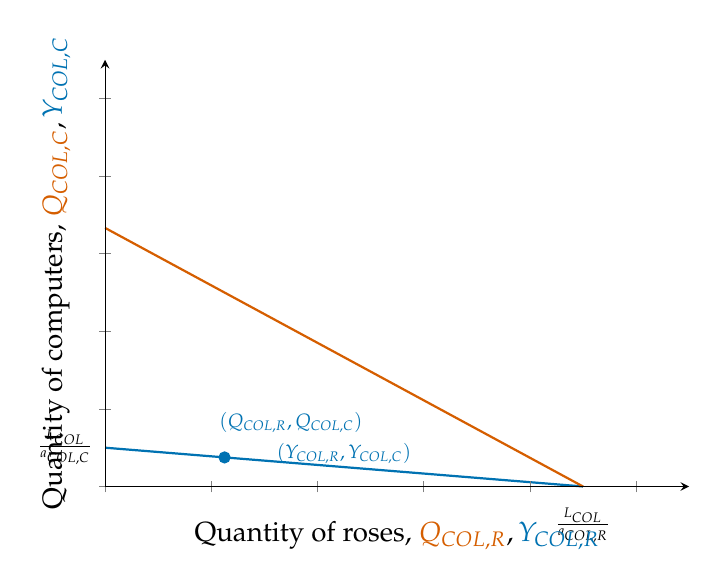
\begin{tikzpicture}
\pgfmathsetmacro{\aC}{900}       % unit labor requirement for computers
\pgfmathsetmacro{\aR}{1}         % unit labor requirement for roses
\pgfmathsetmacro{\alpha}{0.75}    % preference for computers
\pgfmathsetmacro{\Lendow}{9}    % labor endowment

% Compute equilibrium quantities
\pgfmathsetmacro{\Qc}{(\alpha*\Lendow)/\aC}
\pgfmathsetmacro{\Qr}{((1 - \alpha)*\Lendow)/\aR}

% Compute utility level
\pgfmathsetmacro{\U}{(\Qc^(\alpha))*(\Qr^(1 - \alpha))}

% Compute prefactor for indifference curve: Qc = A * Qr^(- (1 - alpha)/alpha)
\pgfmathsetmacro{\expo}{(1 - \alpha)/\alpha}
\pgfmathsetmacro{\A}{\U^(1/\alpha)}

\centering
\begin{axis}[
    ylabel={Quantity of computers, $\textcolor{red}{Q_{COL,C}}, \textcolor{blue}{Y_{COL,C}}$},
    xlabel={Quantity of roses, $\textcolor{red}{Q_{COL,R}}, \textcolor{blue}{Y_{COL,R}}$},
    ymin=0, ymax=0.11,
    xmin=0, xmax=11,
    yticklabel=\empty,
    xticklabel=\empty,
    axis lines=left,
    enlargelimits=false,
    clip=false,
    axis on top,
    scaled x ticks=false,
    width=9cm, height=7cm,
    title style={font=\bfseries}
]

% PPF: Q_C = (L/a_C) - (a_R/a_C) * Q_R
\addplot[thick, blue, domain=0:9] {\Lendow/\aC - (\aR/\aC)*x};

\addplot[thick, red, domain=0:9] {1/15 - (1/135)*x};


% Indifference curve through optimal bundle
%\addplot[red, domain=0.1:9, samples=100] {\A * x^(-\expo)};

% Labels

%\node at (axis cs:3.5,0.03) {\Large $\mathcal{Y}_{US}$};
\node at (axis cs:\Lendow/\aR,-.01) {\scriptsize $\frac{L_{COL}}{a_{COL,R}}$};
\node at (axis cs:-.75,\Lendow/\aC) {\scriptsize $\frac{L_{COL}}{a_{COL,C}}$};


% Equilibrium point
\addplot[only marks, mark=*, color=blue, mark size=2pt] coordinates {(\Qr, \Qc)};
\node at (axis cs:\Qr + 1.25,\Qc + 0.009) {\scriptsize $\textcolor{blue}{(Q_{COL,R},Q_{COL,C})}$};
\node at (axis cs:\Qr + 2.25,\Qc + 0.001) {\scriptsize $\textcolor{blue}{(Y_{COL,R},Y_{COL,C})}$};

\end{axis}

\end{tikzpicture}
}

\end{subfigure}

\caption{Autarky Equilibrium + Trade Prices}
\end{figure}
\end{center}
\end{frame}


\begin{frame}{Production Possibilities Frontier + Trade Prices + Specialization}
\begin{center}

\begin{figure}[htbp]

% California
\begin{subfigure}{}
\resizebox{0.48\linewidth}{!}{%
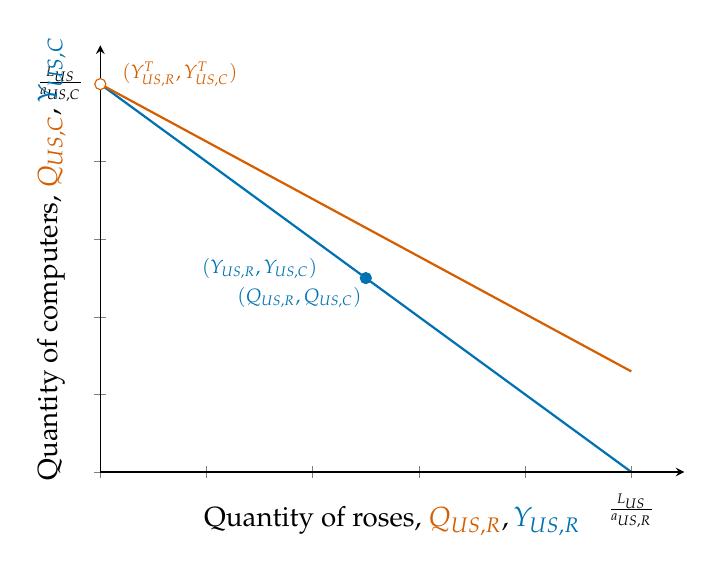
\begin{tikzpicture}
\pgfmathsetmacro{\aC}{100}       % unit labor requirement for computers
\pgfmathsetmacro{\aR}{1}         % unit labor requirement for roses
\pgfmathsetmacro{\alpha}{0.5}    % preference for computers
\pgfmathsetmacro{\Lendow}{10}    % labor endowment

% Compute equilibrium quantities
\pgfmathsetmacro{\Qc}{(\alpha*\Lendow)/\aC}
\pgfmathsetmacro{\Qr}{((1 - \alpha)*\Lendow)/\aR}

% Compute utility level
\pgfmathsetmacro{\U}{(\Qc^(\alpha))*(\Qr^(1 - \alpha))}

% Compute prefactor for indifference curve: Qc = A * Qr^(- (1 - alpha)/alpha)
\pgfmathsetmacro{\expo}{(1 - \alpha)/\alpha}
\pgfmathsetmacro{\A}{\U^(1/\alpha)}

\centering
\begin{axis}[
    ylabel={Quantity of computers, $\textcolor{red}{Q_{US,C}}, \textcolor{blue}{Y_{US,C}}$},
    xlabel={Quantity of roses, $\textcolor{red}{Q_{US,R}}, \textcolor{blue}{Y_{US,R}}$},
    ymin=0, ymax=0.11,
    xmin=0, xmax=11,
    yticklabel=\empty,
    xticklabel=\empty,
    axis lines=left,
    enlargelimits=false,
    clip=false,
    axis on top,
    scaled x ticks=false,
    width=9cm, height=7cm,
    title style={font=\bfseries}
]

% PPF: Q_C = (L/a_C) - (a_R/a_C) * Q_R
\addplot[thick, blue, domain=0:10] {\Lendow/\aC - (\aR/\aC)*x};

\addplot[thick, red, domain=0:10] {\Lendow/\aC - (1/135)*x};


% Indifference curve through optimal bundle
%\addplot[red, domain=0.1:9, samples=100] {\A * x^(-\expo)};

% Labels

%\node at (axis cs:3.5,0.03) {\Large $\mathcal{Y}_{US}$};
\node at (axis cs:\Lendow/\aR,-.01) {\scriptsize $\frac{L_{US}}{a_{US,R}}$};
\node at (axis cs:-.75,\Lendow/\aC) {\scriptsize $\frac{L_{US}}{a_{US,C}}$};


% Equilibrium point
\addplot[only marks, mark=*, color=blue, mark size=2pt] coordinates {(\Qr, \Qc)};
\node at (axis cs:\Qr - 1.25,\Qc - 0.005) {\scriptsize $\textcolor{blue}{(Q_{US,R},Q_{US,C})}$};
\node at (axis cs:\Qr - 2,\Qc + 0.0025) {\scriptsize $\textcolor{blue}{(Y_{US,R},Y_{US,C})}$};

\addplot[only marks, mark=*, mark options={fill=white, draw=red}, mark size=2pt] coordinates {(0, \Lendow/\aC)};
\node at (axis cs:0 + 1.5,\Lendow/\aC + 0.0025) {\scriptsize $\textcolor{red}{(Y^T_{US,R},Y^T_{US,C})}$};

\end{axis}

\end{tikzpicture}
}
\end{subfigure}
%
% Colombia
\begin{subfigure}{}
\resizebox{0.48\linewidth}{!}{%
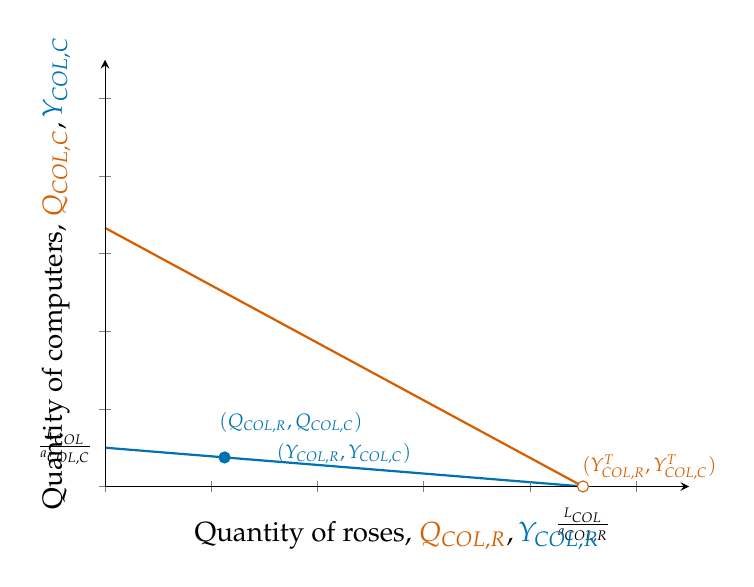
\begin{tikzpicture}
\pgfmathsetmacro{\aC}{900}       % unit labor requirement for computers
\pgfmathsetmacro{\aR}{1}         % unit labor requirement for roses
\pgfmathsetmacro{\alpha}{0.75}    % preference for computers
\pgfmathsetmacro{\Lendow}{9}    % labor endowment

% Compute equilibrium quantities
\pgfmathsetmacro{\Qc}{(\alpha*\Lendow)/\aC}
\pgfmathsetmacro{\Qr}{((1 - \alpha)*\Lendow)/\aR}

% Compute utility level
\pgfmathsetmacro{\U}{(\Qc^(\alpha))*(\Qr^(1 - \alpha))}

% Compute prefactor for indifference curve: Qc = A * Qr^(- (1 - alpha)/alpha)
\pgfmathsetmacro{\expo}{(1 - \alpha)/\alpha}
\pgfmathsetmacro{\A}{\U^(1/\alpha)}

\centering
\begin{axis}[
    ylabel={Quantity of computers, $\textcolor{red}{Q_{COL,C}}, \textcolor{blue}{Y_{COL,C}}$},
    xlabel={Quantity of roses, $\textcolor{red}{Q_{COL,R}}, \textcolor{blue}{Y_{COL,R}}$},
    ymin=0, ymax=0.11,
    xmin=0, xmax=11,
    yticklabel=\empty,
    xticklabel=\empty,
    axis lines=left,
    enlargelimits=false,
    clip=false,
    axis on top,
    scaled x ticks=false,
    width=9cm, height=7cm,
    title style={font=\bfseries}
]

% PPF: Q_C = (L/a_C) - (a_R/a_C) * Q_R
\addplot[thick, blue, domain=0:9] {\Lendow/\aC - (\aR/\aC)*x};

\addplot[thick, red, domain=0:9] {1/15 - (1/135)*x};


% Indifference curve through optimal bundle
%\addplot[red, domain=0.1:9, samples=100] {\A * x^(-\expo)};

% Labels

%\node at (axis cs:3.5,0.03) {\Large $\mathcal{Y}_{US}$};
\node at (axis cs:\Lendow/\aR,-.01) {\scriptsize $\frac{L_{COL}}{a_{COL,R}}$};
\node at (axis cs:-.75,\Lendow/\aC) {\scriptsize $\frac{L_{COL}}{a_{COL,C}}$};


% Equilibrium point
\addplot[only marks, mark=*, color=blue, mark size=2pt] coordinates {(\Qr, \Qc)};
\node at (axis cs:\Qr + 1.25,\Qc + 0.009) {\scriptsize $\textcolor{blue}{(Q_{COL,R},Q_{COL,C})}$};
\node at (axis cs:\Qr + 2.25,\Qc + 0.001) {\scriptsize $\textcolor{blue}{(Y_{COL,R},Y_{COL,C})}$};

\addplot[only marks, mark=*, mark options={fill=white, draw=red}, mark size=2pt] coordinates {(\Lendow/\aR, 0)};
\node at (axis cs:\Lendow/\aR + 1.25,0 + 0.005) {\scriptsize $\textcolor{red}{(Y^T_{COL,R},Y^T_{COL,C})}$};

\end{axis}

\end{tikzpicture}
}

\end{subfigure}

\caption{Production under Free Trade induces Specialization}

\end{figure}
\end{center}
\end{frame}

\section{Demand and trade balance}

\begin{frame}{Optimal demands under free trade}
\begin{wideitemize}
    \item Recall $w_{US} = P_{C} / a_{US,C}, \quad w_{COL} = P_{R} / a_{COL,R}, \quad  P_C/P_R = 135$
    \item<2-> Demand functions:    
  \onslide<2->{ \scriptsize
  \begin{equation*}
    Q^T_{US,C} = \alpha_{US} \frac{w_{US }L_{US} }{P_{C}} = \alpha_{US} \frac{L_{US} }{a_{US,C}} = 1/2 \times \frac{300 \text{m}}{100{,}000} = 50,000
    \end{equation*}
    }
    \onslide<3->{ \scriptsize
     \begin{equation*}
    Q^T_{COL,C} = \alpha_{COL} \frac{w_{COL }L_{COL} }{P_{C}} = \alpha_{COL} \frac{L_{COL} }{a_{COL,R} \times P_C/P_R} = 3/4 \times \frac{54 \text{m}}{6 \times 135} = 50,000
    \end{equation*}
    }
    \onslide<4->{ \scriptsize
    \begin{equation*}        
    Q^T_{US,R} = (1- \alpha_{US})   \frac{W_{US} L_{US} }{P_R} = (1- \alpha_{US})   \frac{P_C}{P_R} \times \frac{L_{US} }{a_{US,C}} = 1/2 \times 135 \times \frac{300 \text{m}}{100{,}000} = 6,750,000
    \end{equation*}
    }
    \onslide<5->{ \scriptsize
    \begin{equation*}
    \qquad Q^T_{COL,R} &=& (1-\alpha_{COL}) \frac{w_{COL} L_{COL} }{P_{R} } = (1-\alpha_{COL}) \frac{L_{COL} }{a_{COL,R} } = 1/4 \times \frac{54 \text{m}}{6} = 2,250,000
    \end{equation*}
    }
    \item<6-> Exports/imports of computers: $Y_{US,C} - Q^T_{US,C} = 100{,}000 - 50{,}000 = 50{,}000 = Q^T_{COL,C}$
    \item<7-> Exports/imports of roses: $Y_{US,R} - Q^T_{US,R} = 9m - 2.25m = 6.75m = Q^T_{US,R}$
\end{wideitemize}


\end{frame}

\begin{frame}{Trade Equilibrium}
\begin{center}


\begin{figure}[htbp]

% California
\begin{subfigure}{}
\resizebox{0.48\linewidth}{!}{%
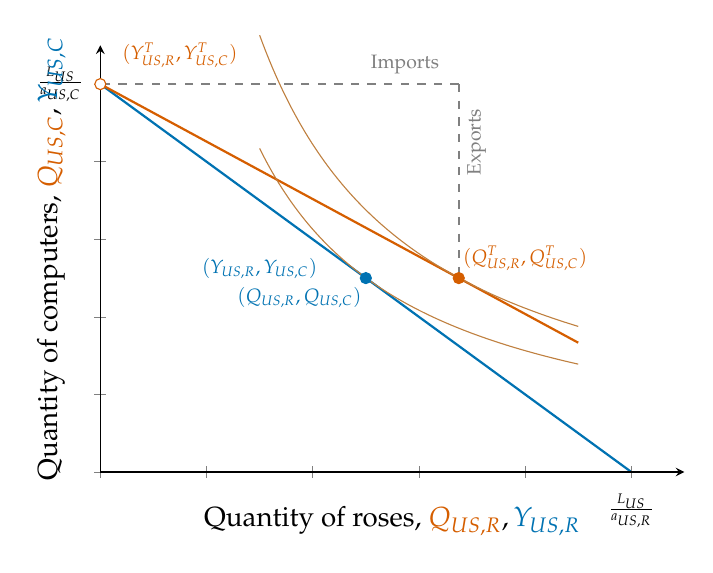
\begin{tikzpicture}
\pgfmathsetmacro{\aC}{100}       % unit labor requirement for computers
\pgfmathsetmacro{\aR}{1}         % unit labor requirement for roses
\pgfmathsetmacro{\alpha}{0.5}    % preference for computers
\pgfmathsetmacro{\Lendow}{10}    % labor endowment
\pgfmathsetmacro{\p}{135}    % trade price

% Compute equilibrium quantities
\pgfmathsetmacro{\Qc}{(\alpha*\Lendow)/\aC}
\pgfmathsetmacro{\Qr}{((1 - \alpha)*\Lendow)/\aR}
\pgfmathsetmacro{\QcT}{(\alpha*\Lendow)/\aC}
\pgfmathsetmacro{\QrT}{((1 - \alpha)*\p*\Lendow)/\aC}

% Compute utility level
\pgfmathsetmacro{\U}{(\Qc^(\alpha))*(\Qr^(1 - \alpha))}
\pgfmathsetmacro{\UT}{(\QcT^(\alpha))*(\QrT^(1 - \alpha))}

% Compute prefactor for indifference curve: Qc = A * Qr^(- (1 - alpha)/alpha)
\pgfmathsetmacro{\expo}{(1 - \alpha)/\alpha}
\pgfmathsetmacro{\A}{\U^(1/\alpha)}
\pgfmathsetmacro{\AT}{\UT^(1/\alpha)}

\centering
\begin{axis}[
    ylabel={Quantity of computers, $\textcolor{red}{Q_{US,C}}, \textcolor{blue}{Y_{US,C}}$},
    xlabel={Quantity of roses, $\textcolor{red}{Q_{US,R}}, \textcolor{blue}{Y_{US,R}}$},
    ymin=0, ymax=\Lendow/\aC * 1.1,
    xmin=0, xmax=\Lendow/\aR * 1.1,
    yticklabel=\empty,
    xticklabel=\empty,
    axis lines=left,
    enlargelimits=false,
    clip=false,
    axis on top,
    scaled x ticks=false,
    width=9cm, height=7cm,
    title style={font=\bfseries}
]

% PPF: Q_C = (L/a_C) - (a_R/a_C) * Q_R
\addplot[thick, blue, domain=0:10] {\Lendow/\aC - (\aR/\aC)*x};
\addplot[thick, red, domain=0:9] {\Lendow/\aC  - (1/\p)*x};

% Indifference curve through optimal bundle
\addplot[brown, domain=3:9, samples=100] {\A * x^(-\expo)};
\addplot[brown, domain=3:9, samples=100] {\AT * x^(-\expo)};

% Labels

%\node at (axis cs:3.5,0.03) {\Large $\mathcal{Y}_{US}$};
\node at (axis cs:\Lendow/\aR,-.01) {\scriptsize $\frac{L_{US}}{a_{US,R}}$};
\node at (axis cs:-.75,\Lendow/\aC) {\scriptsize $\frac{L_{US}}{a_{US,C}}$};

% Equilibrium point
\addplot[only marks, mark=*, color=blue, mark size=2pt] coordinates {(\Qr, \Qc)};
\node at (axis cs:\Qr - 1.25,\Qc - 0.005) {\scriptsize $\textcolor{blue}{(Q_{US,R},Q_{US,C})}$};
\node at (axis cs:\Qr - 2,\Qc + 0.0025) {\scriptsize $\textcolor{blue}{(Y_{US,R},Y_{US,C})}$};

\addplot[only marks, mark=*, color=red, mark size=2pt] coordinates {(\QrT, \QcT)};
\node at (axis cs:\QrT + 1.25,\QcT + 0.005) {\scriptsize $\textcolor{red}{(Q^T_{US,R},Q^T_{US,C})}$};

\addplot[only marks, mark=*, mark options={fill=white, draw=red}, mark size=2pt] coordinates {(0, \Lendow/\aC)};
\node at (axis cs:0 + 1.5,\Lendow/\aC + 0.0075) {\scriptsize $\textcolor{red}{(Y^T_{US,R},Y^T_{US,C})}$};

% Arrows for exports (horizontal)
\draw[-, dashed, thick, gray] 
    (axis cs:\QrT,\Lendow/\aC) -- 
    (axis cs:0,\Lendow/\aC);
\node[gray] at (axis cs:\QrT*0.85,\Lendow/\aC*1.05) {\scriptsize Imports};

% Arrows for imports (vertical)
\draw[-, dashed, thick, gray] 
    (axis cs:\QrT,\Lendow/\aC) -- 
    (axis cs:\QrT, \QcT);
\node[gray, rotate=90] at (axis cs:\QrT*1.05,\Lendow/\aC*0.85) {\scriptsize Exports};



\end{axis}

\end{tikzpicture}
}
\end{subfigure}
%
% Colombia
\begin{subfigure}{}
\resizebox{0.48\linewidth}{!}{%

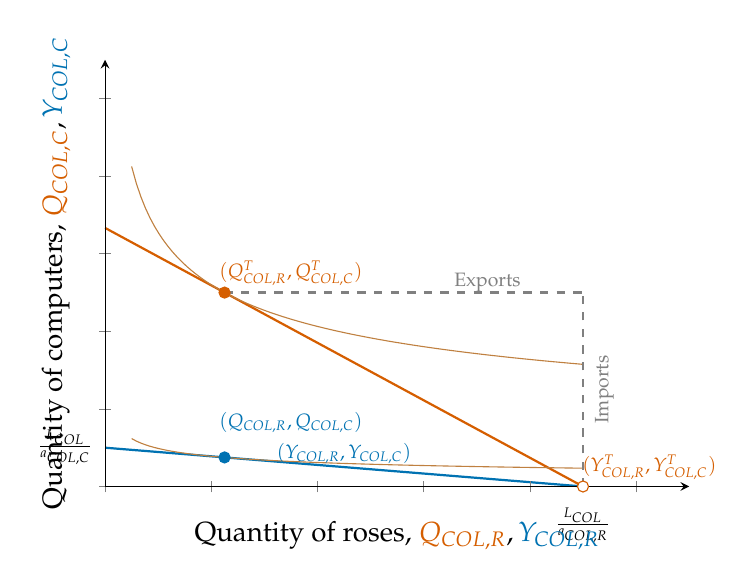
\begin{tikzpicture}
\pgfmathsetmacro{\aC}{900}       % unit labor requirement for computers
\pgfmathsetmacro{\aR}{1}         % unit labor requirement for roses
\pgfmathsetmacro{\alpha}{0.75}    % preference for computers
\pgfmathsetmacro{\Lendow}{9}    % labor endowment
\pgfmathsetmacro{\p}{135}    % trade price


% Compute equilibrium quantities
\pgfmathsetmacro{\Qc}{(\alpha*\Lendow)/\aC}
\pgfmathsetmacro{\Qr}{((1 - \alpha)*\Lendow)/\aR}
\pgfmathsetmacro{\QcT}{(\alpha*\Lendow)/(\aR*\p)}
\pgfmathsetmacro{\QrT}{((1 - \alpha)*\Lendow)/\aR}

% Compute prefactor for indifference curve: Qc = A * Qr^(- (1 - alpha)/alpha)
\pgfmathsetmacro{\expo}{(1 - \alpha)/\alpha}
\pgfmathsetmacro{\A}{\Qc * \Qr^((1 - \alpha)/\alpha))}
\pgfmathsetmacro{\AT}{\QcT * \QrT^((1 - \alpha)/\alpha))}

\centering
\begin{axis}[
    ylabel={Quantity of computers, $\textcolor{red}{Q_{COL,C}}, \textcolor{blue}{Y_{COL,C}}$},
    xlabel={Quantity of roses, $\textcolor{red}{Q_{COL,R}}, \textcolor{blue}{Y_{COL,R}}$},
    ymin=0, ymax=0.11,
    xmin=0, xmax=11,
    yticklabel=\empty,
    xticklabel=\empty,
    axis lines=left,
    enlargelimits=false,
    clip=false,
    axis on top,
    scaled x ticks=false,
    width=9cm, height=7cm,
    title style={font=\bfseries}
]

% PPF: Q_C = (L/a_C) - (a_R/a_C) * Q_R
\addplot[thick, blue, domain=0:9] {\Lendow/\aC - (\aR/\aC)*x};
\addplot[thick, red, domain=0:9] {\Lendow/\aR * 1/ \p - (1/\p)*x};


% Indifference curve through optimal bundle
\addplot[brown, domain=0.5:9, samples=100] {\A * x^(-\expo)};
\addplot[brown, domain=0.5:9, samples=100] {\AT * x^(-\expo)};

% Labels

%\node at (axis cs:3.5,0.03) {\Large $\mathcal{Y}_{US}$};
\node at (axis cs:\Lendow/\aR,-.01) {\scriptsize $\frac{L_{COL}}{a_{COL,R}}$};
\node at (axis cs:-.75,\Lendow/\aC) {\scriptsize $\frac{L_{COL}}{a_{COL,C}}$};


% Equilibrium point
\addplot[only marks, mark=*, color=blue, mark size=2pt] coordinates {(\Qr, \Qc)};
\node at (axis cs:\Qr + 1.25,\Qc + 0.009) {\scriptsize $\textcolor{blue}{(Q_{COL,R},Q_{COL,C})}$};
\node at (axis cs:\Qr + 2.25,\Qc + 0.001) {\scriptsize $\textcolor{blue}{(Y_{COL,R},Y_{COL,C})}$};


\addplot[only marks, mark=*, color=red, mark size=2pt] coordinates {(\QrT, \QcT)};
\node at (axis cs:\QrT + 1.25,\QcT + 0.005) {\scriptsize $\textcolor{red}{(Q^T_{COL,R},Q^T_{COL,C})}$};

\addplot[only marks, mark=*, mark options={fill=white, draw=red}, mark size=2pt] coordinates {(\Lendow/\aR, 0)};
\node at (axis cs:\Lendow/\aR + 1.25,0 + 0.005) {\scriptsize $\textcolor{red}{(Y^T_{COL,R},Y^T_{COL,C})}$};

% Arrows for exports (horizontal)
\draw[-, dashed, thick, gray] 
    (axis cs:\QrT,\QcT) -- 
    (axis cs:\Lendow/\aR,\QcT);
\node[gray] at (axis cs:{ \Lendow/\aR *0.8}, \QcT*1.05) {\scriptsize Exports};

% Arrows for imports (vertical)
\draw[-, dashed, thick, gray] 
    (axis cs:{\Lendow/\aR},0) -- 
    (axis cs:{\Lendow/\aR}, \QcT);
\node[gray, rotate=90] at (axis cs:{\Lendow/\aR + 0.4}, {\QcT/2}) {\scriptsize Imports};

\end{axis}

\end{tikzpicture}
}

\end{subfigure}

\caption{Specialization + Trade Equilibrium}

\end{figure}

\end{center}
\end{frame}

\section{Epilogue}

\begin{frame}{Some misconceptions about comparative advantage}
\begin{wideitemize}
    \item ``Free trade is only beneficial if a country is productive enough to compete.'' \\
    \qquad No. Trade is beneficial if there is a comparative advantage. Absolute disadvantage does not matter.

        \item ``Free trade lowers income in low-wage countries.'' \\
    \qquad No. Trade is beneficial if there is a comparative advantage. Absolute wages do not matter.

    \item ``Free trade makes us poorer because we spend money on other countries goods.'' \\
    \qquad No. Having access to more affordable goods makes us better off by specializing and trading.

    \item ``Free trade closes the income gap between poor and rich countries.'' \\
    \qquad No. Trade raises every country’s welfare beyond autarky welfare. Per capita
income differences remain, and depend on a country’s production possibilities.

\end{wideitemize}
    
\end{frame}

\begin{frame}{Is free trade always ideal?}
\begin{wideitemize}
    \item This model is quite simple. Some things it does not consider:

    \begin{itemize}
        \item \blue{Increasing returns to scale}: a country may be competitive in an industry but it requires large initial investment (R\&D, ships, planes, etc) -- temporary protection?

        \item \blue{Distributional effects}: even if a country benefits in the aggregate, it could be the case that vulnerable groups are very exposed, increasing inequality

        \item \blue{Price manipulation}: if a country is very large relative to the world, it may be able to manipulate the purchase price in its favor using tariffs
        
        \item \blue{Environmental externalities}: trade policy can be an instrument to internalize some ``bads'' to the price of ``goods''
        \end{itemize}

\end{wideitemize}
    
\end{frame}


\end{document}
